
%% $Id$

\documentclass[12pt,a4paper]{report}
\usepackage{latexsym}
\usepackage{amssymb}
\usepackage[english]{babel}
\usepackage[latin1]{inputenc}
\usepackage[only,bigsqcap]{stmaryrd}
\usepackage{wasysym}
\usepackage{textcomp}
\let\RightarrowOrig=\Rightarrow\usepackage{marvosym}\let\Rightarrow=\RightarrowOrig  %bug in marvosym!?
\usepackage{supertabular}
\let\intorig=\int  %iman.sty redefines \int
\usepackage{graphicx,../iman,../extra,../ttbox,../../Distribution/lib/texinputs/isabelle,../../Distribution/lib/texinputs/isabellesym,../pdfsetup}

\isabellestyle{it}

\title{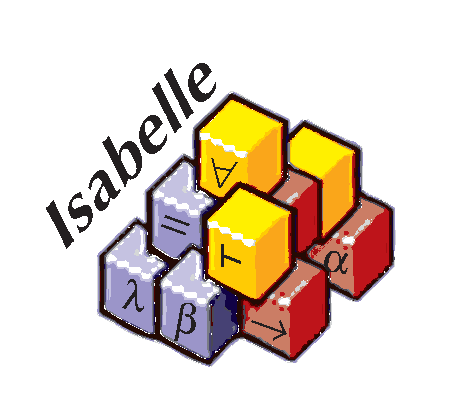
\includegraphics[scale=0.5]{isabelle} \\[4ex] The Isabelle System Manual}

\author{\emph{Markus Wenzel} and \emph{Stefan Berghofer} \\
  TU M\"unchen}

\makeindex

\setcounter{secnumdepth}{1} \setcounter{tocdepth}{2}

\pagestyle{headings}
\sloppy
\binperiod     %%%treat . like a binary operator

\begin{document}

\underscoreoff

\maketitle 
\pagenumbering{roman} \tableofcontents \clearfirst

\chapter{The Basics}

\section{Introduction}

This book is a tutorial on how to use the theorem prover Isabelle/HOL as a
specification and verification system. Isabelle is a generic system for
implementing logical formalisms, and Isabelle/HOL is the specialization
of Isabelle for HOL, which abbreviates Higher-Order Logic. We introduce
HOL step by step following the equation
\[ \mbox{HOL} = \mbox{Functional Programming} + \mbox{Logic}. \]
We do not assume that you are familiar with mathematical logic. 
However, we do assume that
you are used to logical and set theoretic notation, as covered
in a good discrete mathematics course~\cite{Rosen-DMA}, and
that you are familiar with the basic concepts of functional
programming~\cite{Bird-Haskell,Hudak-Haskell,paulson-ml2,Thompson-Haskell}.
Although this tutorial initially concentrates on functional programming, do
not be misled: HOL can express most mathematical concepts, and functional
programming is just one particularly simple and ubiquitous instance.

Isabelle~\cite{paulson-isa-book} is implemented in ML~\cite{SML}.  This has
influenced some of Isabelle/HOL's concrete syntax but is otherwise irrelevant
for us: this tutorial is based on
Isabelle/Isar~\cite{isabelle-isar-ref}, an extension of Isabelle which hides
the implementation language almost completely.  Thus the full name of the
system should be Isabelle/Isar/HOL, but that is a bit of a mouthful.

There are other implementations of HOL, in particular the one by Mike Gordon
\index{Gordon, Mike}%
\emph{et al.}, which is usually referred to as ``the HOL system''
\cite{mgordon-hol}. For us, HOL refers to the logical system, and sometimes
its incarnation Isabelle/HOL\@.

A tutorial is by definition incomplete.  Currently the tutorial only
introduces the rudiments of Isar's proof language. To fully exploit the power
of Isar, in particular the ability to write readable and structured proofs,
you need to consult the Isabelle/Isar Reference
Manual~\cite{isabelle-isar-ref} and Wenzel's PhD thesis~\cite{Wenzel-PhD}
which discusses many proof patterns. If you want to use Isabelle's ML level
directly (for example for writing your own proof procedures) see the Isabelle
Reference Manual~\cite{isabelle-ref}; for details relating to HOL see the
Isabelle/HOL manual~\cite{isabelle-HOL}. All manuals have a comprehensive
index.

\section{Theories}
\label{sec:Basic:Theories}

\index{theories|(}%
Working with Isabelle means creating theories. Roughly speaking, a
\textbf{theory} is a named collection of types, functions, and theorems,
much like a module in a programming language or a specification in a
specification language. In fact, theories in HOL can be either. The general
format of a theory \texttt{T} is
\begin{ttbox}
theory T
imports B\(@1\) \(\ldots\) B\(@n\)
begin
{\rmfamily\textit{declarations, definitions, and proofs}}
end
\end{ttbox}\cmmdx{theory}\cmmdx{imports}
where \texttt{B}$@1$ \dots\ \texttt{B}$@n$ are the names of existing
theories that \texttt{T} is based on and \textit{declarations,
    definitions, and proofs} represents the newly introduced concepts
(types, functions etc.) and proofs about them. The \texttt{B}$@i$ are the
direct \textbf{parent theories}\indexbold{parent theories} of~\texttt{T}\@.
Everything defined in the parent theories (and their parents, recursively) is
automatically visible. To avoid name clashes, identifiers can be
\textbf{qualified}\indexbold{identifiers!qualified}
by theory names as in \texttt{T.f} and~\texttt{B.f}. 
Each theory \texttt{T} must
reside in a \textbf{theory file}\index{theory files} named \texttt{T.thy}.

This tutorial is concerned with introducing you to the different linguistic
constructs that can fill the \textit{declarations, definitions, and
    proofs} above.  A complete grammar of the basic
constructs is found in the Isabelle/Isar Reference
Manual~\cite{isabelle-isar-ref}.

HOL's theory collection is available online at
\begin{center}\small
    \url{http://isabelle.in.tum.de/library/HOL/}
\end{center}
and is recommended browsing. Note that most of the theories 
are based on classical Isabelle without the Isar extension. This means that
they look slightly different than the theories in this tutorial, and that all
proofs are in separate ML files.

\begin{warn}
  HOL contains a theory \thydx{Main}, the union of all the basic
  predefined theories like arithmetic, lists, sets, etc.  
  Unless you know what you are doing, always include \isa{Main}
  as a direct or indirect parent of all your theories.
\end{warn}
There is also a growing Library~\cite{HOL-Library}\index{Library}
of useful theories that are not part of \isa{Main} but can be included
among the parents of a theory and will then be loaded automatically.%
\index{theories|)}


\section{Types, Terms and Formulae}
\label{sec:TypesTermsForms}

Embedded in a theory are the types, terms and formulae of HOL\@. HOL is a typed
logic whose type system resembles that of functional programming languages
like ML or Haskell. Thus there are
\index{types|(}
\begin{description}
\item[base types,] 
in particular \tydx{bool}, the type of truth values,
and \tydx{nat}, the type of natural numbers.
\item[type constructors,]\index{type constructors}
 in particular \tydx{list}, the type of
lists, and \tydx{set}, the type of sets. Type constructors are written
postfix, e.g.\ \isa{(nat)list} is the type of lists whose elements are
natural numbers. Parentheses around single arguments can be dropped (as in
\isa{nat list}), multiple arguments are separated by commas (as in
\isa{(bool,nat)ty}).
\item[function types,]\index{function types}
denoted by \isasymFun\indexbold{$IsaFun@\isasymFun}.
  In HOL \isasymFun\ represents \emph{total} functions only. As is customary,
  \isa{$\tau@1$ \isasymFun~$\tau@2$ \isasymFun~$\tau@3$} means
  \isa{$\tau@1$ \isasymFun~($\tau@2$ \isasymFun~$\tau@3$)}. Isabelle also
  supports the notation \isa{[$\tau@1,\dots,\tau@n$] \isasymFun~$\tau$}
  which abbreviates \isa{$\tau@1$ \isasymFun~$\cdots$ \isasymFun~$\tau@n$
    \isasymFun~$\tau$}.
\item[type variables,]\index{type variables}\index{variables!type}
  denoted by \ttindexboldpos{'a}{$Isatype}, \isa{'b} etc., just like in ML\@. They give rise
  to polymorphic types like \isa{'a \isasymFun~'a}, the type of the identity
  function.
\end{description}
\begin{warn}
  Types are extremely important because they prevent us from writing
  nonsense.  Isabelle insists that all terms and formulae must be well-typed
  and will print an error message if a type mismatch is encountered. To
  reduce the amount of explicit type information that needs to be provided by
  the user, Isabelle infers the type of all variables automatically (this is
  called \bfindex{type inference}) and keeps quiet about it. Occasionally
  this may lead to misunderstandings between you and the system. If anything
  strange happens, we recommend that you set the flag\index{flags}
  \isa{show_types}\index{*show_types (flag)}.  
  Isabelle will then display type information
  that is usually suppressed.  Simply type
\begin{ttbox}
ML "set show_types"
\end{ttbox}

\noindent
This can be reversed by \texttt{ML "reset show_types"}. Various other flags,
which we introduce as we go along, can be set and reset in the same manner.%
\index{flags!setting and resetting}
\end{warn}%
\index{types|)}


\index{terms|(}
\textbf{Terms} are formed as in functional programming by
applying functions to arguments. If \isa{f} is a function of type
\isa{$\tau@1$ \isasymFun~$\tau@2$} and \isa{t} is a term of type
$\tau@1$ then \isa{f~t} is a term of type $\tau@2$. HOL also supports
infix functions like \isa{+} and some basic constructs from functional
programming, such as conditional expressions:
\begin{description}
\item[\isa{if $b$ then $t@1$ else $t@2$}]\index{*if expressions}
Here $b$ is of type \isa{bool} and $t@1$ and $t@2$ are of the same type.
\item[\isa{let $x$ = $t$ in $u$}]\index{*let expressions}
is equivalent to $u$ where all free occurrences of $x$ have been replaced by
$t$. For example,
\isa{let x = 0 in x+x} is equivalent to \isa{0+0}. Multiple bindings are separated
by semicolons: \isa{let $x@1$ = $t@1$;\dots; $x@n$ = $t@n$ in $u$}.
\item[\isa{case $e$ of $c@1$ \isasymFun~$e@1$ |~\dots~| $c@n$ \isasymFun~$e@n$}]
\index{*case expressions}
evaluates to $e@i$ if $e$ is of the form $c@i$.
\end{description}

Terms may also contain
\isasymlambda-abstractions.\index{lambda@$\lambda$ expressions}
For example,
\isa{\isasymlambda{}x.~x+1} is the function that takes an argument \isa{x} and
returns \isa{x+1}. Instead of
\isa{\isasymlambda{}x.\isasymlambda{}y.\isasymlambda{}z.~$t$} we can write
\isa{\isasymlambda{}x~y~z.~$t$}.%
\index{terms|)}

\index{formulae|(}%
\textbf{Formulae} are terms of type \tydx{bool}.
There are the basic constants \cdx{True} and \cdx{False} and
the usual logical connectives (in decreasing order of priority):
\indexboldpos{\protect\isasymnot}{$HOL0not}, \indexboldpos{\protect\isasymand}{$HOL0and},
\indexboldpos{\protect\isasymor}{$HOL0or}, and \indexboldpos{\protect\isasymimp}{$HOL0imp},
all of which (except the unary \isasymnot) associate to the right. In
particular \isa{A \isasymimp~B \isasymimp~C} means \isa{A \isasymimp~(B
  \isasymimp~C)} and is thus logically equivalent to \isa{A \isasymand~B
  \isasymimp~C} (which is \isa{(A \isasymand~B) \isasymimp~C}).

Equality\index{equality} is available in the form of the infix function
\isa{=} of type \isa{'a \isasymFun~'a
  \isasymFun~bool}. Thus \isa{$t@1$ = $t@2$} is a formula provided $t@1$
and $t@2$ are terms of the same type. If $t@1$ and $t@2$ are of type
\isa{bool} then \isa{=} acts as \rmindex{if-and-only-if}.
The formula
\isa{$t@1$~\isasymnoteq~$t@2$} is merely an abbreviation for
\isa{\isasymnot($t@1$ = $t@2$)}.

Quantifiers\index{quantifiers} are written as
\isa{\isasymforall{}x.~$P$} and \isa{\isasymexists{}x.~$P$}. 
There is even
\isa{\isasymuniqex{}x.~$P$}, which
means that there exists exactly one \isa{x} that satisfies \isa{$P$}. 
Nested quantifications can be abbreviated:
\isa{\isasymforall{}x~y~z.~$P$} means
\isa{\isasymforall{}x.\isasymforall{}y.\isasymforall{}z.~$P$}.%
\index{formulae|)}

Despite type inference, it is sometimes necessary to attach explicit
\bfindex{type constraints} to a term.  The syntax is
\isa{$t$::$\tau$} as in \isa{x < (y::nat)}. Note that
\ttindexboldpos{::}{$Isatype} binds weakly and should therefore be enclosed
in parentheses.  For instance,
\isa{x < y::nat} is ill-typed because it is interpreted as
\isa{(x < y)::nat}.  Type constraints may be needed to disambiguate
expressions
involving overloaded functions such as~\isa{+}, 
\isa{*} and~\isa{<}.  Section~\ref{sec:overloading} 
discusses overloading, while Table~\ref{tab:overloading} presents the most
important overloaded function symbols.

In general, HOL's concrete \rmindex{syntax} tries to follow the conventions of
functional programming and mathematics.  Here are the main rules that you
should be familiar with to avoid certain syntactic traps:
\begin{itemize}
\item
Remember that \isa{f t u} means \isa{(f t) u} and not \isa{f(t u)}!
\item
Isabelle allows infix functions like \isa{+}. The prefix form of function
application binds more strongly than anything else and hence \isa{f~x + y}
means \isa{(f~x)~+~y} and not \isa{f(x+y)}.
\item Remember that in HOL if-and-only-if is expressed using equality.  But
  equality has a high priority, as befitting a relation, while if-and-only-if
  typically has the lowest priority.  Thus, \isa{\isasymnot~\isasymnot~P =
    P} means \isa{\isasymnot\isasymnot(P = P)} and not
  \isa{(\isasymnot\isasymnot P) = P}. When using \isa{=} to mean
  logical equivalence, enclose both operands in parentheses, as in \isa{(A
    \isasymand~B) = (B \isasymand~A)}.
\item
Constructs with an opening but without a closing delimiter bind very weakly
and should therefore be enclosed in parentheses if they appear in subterms, as
in \isa{(\isasymlambda{}x.~x) = f}.  This includes 
\isa{if},\index{*if expressions}
\isa{let},\index{*let expressions}
\isa{case},\index{*case expressions}
\isa{\isasymlambda}, and quantifiers.
\item
Never write \isa{\isasymlambda{}x.x} or \isa{\isasymforall{}x.x=x}
because \isa{x.x} is always taken as a single qualified identifier. Write
\isa{\isasymlambda{}x.~x} and \isa{\isasymforall{}x.~x=x} instead.
\item Identifiers\indexbold{identifiers} may contain the characters \isa{_} 
and~\isa{'}, except at the beginning.
\end{itemize}

For the sake of readability, we use the usual mathematical symbols throughout
the tutorial. Their \textsc{ascii}-equivalents are shown in table~\ref{tab:ascii} in
the appendix.

\begin{warn}
A particular
problem for novices can be the priority of operators. If you are unsure, use
additional parentheses. In those cases where Isabelle echoes your
input, you can see which parentheses are dropped --- they were superfluous. If
you are unsure how to interpret Isabelle's output because you don't know
where the (dropped) parentheses go, set the flag\index{flags}
\isa{show_brackets}\index{*show_brackets (flag)}:
\begin{ttbox}
ML "set show_brackets"; \(\dots\); ML "reset show_brackets";
\end{ttbox}
\end{warn}


\section{Variables}
\label{sec:variables}
\index{variables|(}

Isabelle distinguishes free and bound variables, as is customary. Bound
variables are automatically renamed to avoid clashes with free variables. In
addition, Isabelle has a third kind of variable, called a \textbf{schematic
  variable}\index{variables!schematic} or \textbf{unknown}\index{unknowns}, 
which must have a~\isa{?} as its first character.  
Logically, an unknown is a free variable. But it may be
instantiated by another term during the proof process. For example, the
mathematical theorem $x = x$ is represented in Isabelle as \isa{?x = ?x},
which means that Isabelle can instantiate it arbitrarily. This is in contrast
to ordinary variables, which remain fixed. The programming language Prolog
calls unknowns {\em logical\/} variables.

Most of the time you can and should ignore unknowns and work with ordinary
variables. Just don't be surprised that after you have finished the proof of
a theorem, Isabelle will turn your free variables into unknowns.  It
indicates that Isabelle will automatically instantiate those unknowns
suitably when the theorem is used in some other proof.
Note that for readability we often drop the \isa{?}s when displaying a theorem.
\begin{warn}
  For historical reasons, Isabelle accepts \isa{?} as an ASCII representation
  of the \(\exists\) symbol.  However, the \isa{?} character must then be followed
  by a space, as in \isa{?~x. f(x) = 0}.  Otherwise, \isa{?x} is
  interpreted as a schematic variable.  The preferred ASCII representation of
  the \(\exists\) symbol is \isa{EX}\@. 
\end{warn}%
\index{variables|)}

\section{Interaction and Interfaces}

Interaction with Isabelle can either occur at the shell level or through more
advanced interfaces. To keep the tutorial independent of the interface, we
have phrased the description of the interaction in a neutral language. For
example, the phrase ``to abandon a proof'' means to type \isacommand{oops} at the
shell level, which is explained the first time the phrase is used. Other
interfaces perform the same act by cursor movements and/or mouse clicks.
Although shell-based interaction is quite feasible for the kind of proof
scripts currently presented in this tutorial, the recommended interface for
Isabelle/Isar is the Emacs-based \bfindex{Proof
  General}~\cite{proofgeneral,Aspinall:TACAS:2000}.

Some interfaces (including the shell level) offer special fonts with
mathematical symbols. For those that do not, remember that \textsc{ascii}-equivalents
are shown in table~\ref{tab:ascii} in the appendix.

Finally, a word about semicolons.\indexbold{$Isar@\texttt{;}} 
Commands may but need not be terminated by semicolons.
At the shell level it is advisable to use semicolons to enforce that a command
is executed immediately; otherwise Isabelle may wait for the next keyword
before it knows that the command is complete.


\section{Getting Started}

Assuming you have installed Isabelle, you start it by typing \texttt{isabelle
  -I HOL} in a shell window.\footnote{Simply executing \texttt{isabelle -I}
  starts the default logic, which usually is already \texttt{HOL}.  This is
  controlled by the \texttt{ISABELLE_LOGIC} setting, see \emph{The Isabelle
    System Manual} for more details.} This presents you with Isabelle's most
basic \textsc{ascii} interface.  In addition you need to open an editor window to
create theory files.  While you are developing a theory, we recommend that you
type each command into the file first and then enter it into Isabelle by
copy-and-paste, thus ensuring that you have a complete record of your theory.
As mentioned above, Proof General offers a much superior interface.
If you have installed Proof General, you can start it by typing \texttt{Isabelle}.


%% $Id$

\chapter{Presenting theories}\label{ch:present}

Isabelle provides several ways to present the outcome of formal developments,
including WWW-based browsable libraries or actual printable documents.
Presentation is centered around the concept of \emph{logic sessions}.  The
global session structure is that of a tree, with Isabelle Pure at its root,
further object-logics derived (e.g.\ HOLCF from HOL, and HOL from Pure), and
application sessions in leaf positions (usually without a separate image).

The \texttt{mkdir} (see \S\ref{sec:tool-mkdir}) and \texttt{make} (see
\S\ref{sec:tool-make}) tools of Isabelle provide the primary means for
managing Isabelle sessions, including proper setup for presentation.  Here the
\texttt{usedir} (see \S\ref{sec:tool-usedir}) tool takes care to let the
\texttt{isabelle} process run any additional stages required for document
preparation, notably the tools \texttt{document} (see
\S\ref{sec:tool-document}) and \texttt{latex} (see \S\ref{sec:tool-latex}).
The complete tool chain for managing batch-mode Isabelle sessions is
illustrated in figure~\ref{fig:session-tools}.

\begin{figure}[htbp]
  \begin{center}
    \begin{tabular}{lp{0.6\textwidth}}
      \texttt{isatool mkdir} & invoked once by the user to create the initial
        source setup (common \texttt{IsaMakefile} plus a single session directory); \\
      \texttt{isatool make} & invoked repeatedly by the user to
        keep session output up-to-date (HTML, documents etc.); \\
      \texttt{isatool usedir} & part of the standard \texttt{IsaMakefile} entry of a session; \\
      \texttt{isabelle} & run through \texttt{isatool usedir}; \\
      \texttt{isatool document} & run by the Isabelle process if document preparation is enabled; \\
      \texttt{isatool latex} & universal {\LaTeX} tool wrapper invoked multiple times
        by \texttt{isatool document}; also useful for manual experiments; \\
    \end{tabular}
    \caption{The tool chain of Isabelle session presentation}
    \label{fig:session-tools}
  \end{center}
\end{figure}


\section{Generating theory browser information} \label{sec:info}
\index{theory browsing information|bold}

As a side-effect of running a logic sessions, Isabelle is able to generate
theory browsing information, including HTML documents that show a theory's
definition, the theorems proved in its ML file and the relationship with its
ancestors and descendants.  Besides the HTML file that is generated for every
theory, Isabelle stores links to all theories in an index file. These indexes
are linked with other indexes to represent the overall tree structure of logic
sessions.

Isabelle also generates graph files that represent the theory hierarchy of a
logic.  There is a graph browser Java applet embedded in the generated HTML
pages, and also a stand-alone application that allows browsing theory graphs
without having to start a WWW client first.  The latter version also includes
features such as generating Postscript files, which are not available in the
applet version.  See \S\ref{sec:browse} for further information.

\medskip

The easiest way to let Isabelle generate theory browsing information for
existing sessions is to append ``\texttt{-i true}'' to the
\settdx{ISABELLE_USEDIR_OPTIONS} before invoking \texttt{isatool make} (or
\texttt{./build} in the distribution).  For example, add something like this
to your Isabelle settings file
\begin{ttbox}
ISABELLE_USEDIR_OPTIONS="-i true"
\end{ttbox}
and then change into the \texttt{src/FOL} directory of the Isabelle
distribution and run \texttt{isatool make}, or even \texttt{isatool make all}.
The presentation output will appear in \texttt{\$ISABELLE_BROWSER_INFO/FOL},
which usually refers to \verb,~/isabelle/browser_info/FOL,.  Note that option
\texttt{-v true} will make the internal runs of \texttt{usedir} more explicit
about such details.

Many standard Isabelle sessions (such as \texttt{HOL/ex}) also provide actual
printable documents.  These are prepared automatically as well if enabled like
this, using the \texttt{-d} option
\begin{ttbox}
ISABELLE_USEDIR_OPTIONS="-i true -d dvi"
\end{ttbox}
Enabling options \texttt{-i} and \texttt{-d} simultaneausly as shown above
causes an appropriate ``document'' link to be included in the HTML index.
Documents (or raw document sources) may be generated independently of browser
information as well, see \S\ref{sec:tool-document} for further details.

\bigskip The theory browsing information is stored in a sub-directory
directory determined by the \settdx{ISABELLE_BROWSER_INFO} setting plus a
prefix corresponding to the session identifier (according to the tree
structure of sub-sessions by default).  A complete WWW view of all standard
object-logics and examples of the Isabelle distribution is available at the
Cambridge or Munich Isabelle sites:
\begin{center}\small
  \begin{tabular}{l}
    \url{http://www.cl.cam.ac.uk/Research/HVG/Isabelle/library/} \\
    \url{http://isabelle.in.tum.de/library/} \\
  \end{tabular}
\end{center}

\medskip In order to present your own theories on the web, simply copy the
corresponding subdirectory from \texttt{ISABELLE_BROWSER_INFO} to your WWW
server, having generated browser info like this:
\begin{ttbox}
isatool usedir -i true HOL Foo
\end{ttbox}
This assumes that directory \texttt{Foo} contains some \texttt{ROOT.ML} file
to load all your theories, and HOL is your parent logic image (\texttt{isatool
  mkdir} assists in setting up Isabelle session directories, see
\S\ref{sec:tool-mkdir}).  Theory browser information for HOL should have been
generated already beforehand.  Alternatively, one may specify an external link
to an existing body of HTML data by giving \texttt{usedir} a \texttt{-P}
option like this:
\begin{ttbox}
isatool usedir -i true -P http://isabelle.in.tum.de/library/ HOL Foo
\end{ttbox}

\medskip For production use, the \texttt{usedir} tool is usually invoked in an
appropriate \texttt{IsaMakefile}, via the Isabelle \texttt{make} utility.
There is a separate \texttt{mkdir} tool to provide easy setup of all this,
with only minimal manual editing required.
\begin{ttbox}
isatool mkdir HOL Foo && isatool make
\end{ttbox}
See \S\ref{sec:tool-mkdir} for more information on preparing Isabelle session
directories, including the setup for documents.


\section{Browsing theory graphs} \label{sec:browse}
\index{theory graph browser|bold} 

The Isabelle graph browser is a general tool for visualizing dependency
graphs.  Certain nodes of the graph (i.e.~theories) can be grouped together in
``directories'', whose contents may be hidden, thus enabling the user to
collapse irrelevant portions of information.  The browser is written in Java,
it can be used both as a stand-alone application and as an applet.  Note that
the option \texttt{-g} of \texttt{isatool usedir} (see
\S\ref{sec:tool-usedir}) creates graph presentations in batch mode for
inclusion in session documents.


\subsection{Invoking the graph browser}

The stand-alone version of the graph browser is wrapped up as an
Isabelle tool called \tooldx{browser}:
\begin{ttbox}
Usage: browser [OPTIONS] [GRAPHFILE]

  Options are:
    -c           cleanup -- remove GRAPHFILE after use
    -o FILE      output to FILE (ps, eps, pdf)
\end{ttbox}
When no filename is specified, the browser automatically changes to the
directory \texttt{ISABELLE_BROWSER_INFO}.

\medskip The \texttt{-c} option causes the input file to be removed after use.

The \texttt{-o} option indicates batch-mode operation, with the output written
to the indicated file; note that \texttt{pdf} produces an \texttt{eps} copy as
well.

\medskip The applet version of the browser is part of the standard WWW theory
presentation, see the link ``theory dependencies'' within each session index.


\subsection{Using the graph browser}

The browser's main window, which is shown in figure
\ref{fig:browserwindow}, consists of two sub-windows: In the left
sub-window, the directory tree is displayed. The graph itself is
displayed in the right sub-window.
\begin{figure}[ht]
  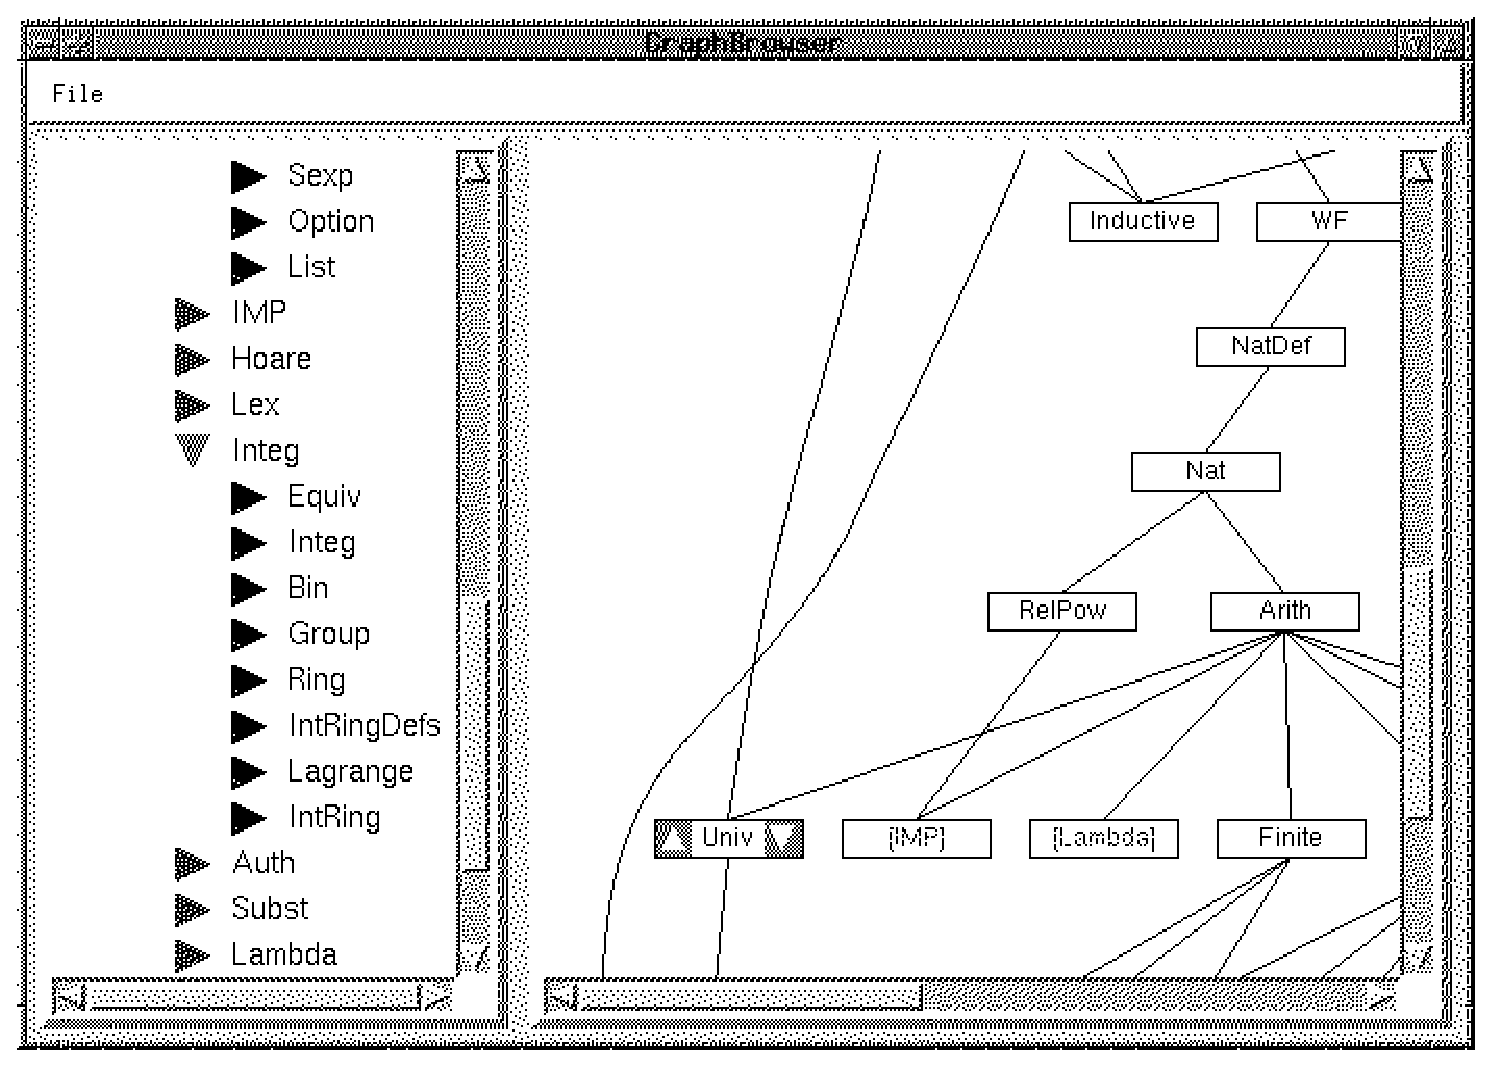
\includegraphics[width=\textwidth]{browser_screenshot}
  \caption{\label{fig:browserwindow} Browser main window}
\end{figure}


\subsubsection*{The directory tree window}

We describe the usage of the directory browser and the meaning of the
different items in the browser window.
\begin{itemize}
  
\item A red arrow before a directory name indicates that the directory
  is currently ``folded'', i.e.~the nodes in this directory are
  collapsed to one single node. In the right sub-window, the names of
  nodes corresponding to folded directories are enclosed in square
  brackets and displayed in red color.
  
\item A green downward arrow before a directory name indicates that
  the directory is currently ``unfolded''. It can be folded by
  clicking on the directory name.  Clicking on the name for a second
  time unfolds the directory again.  Alternatively, a directory can
  also be unfolded by clicking on the corresponding node in the right
  sub-window.
  
\item Blue arrows stand before ordinary node names. When clicking on such a
  name (i.e.\ that of a theory), the graph display window focuses to the
  corresponding node. Double clicking invokes a text viewer window in which
  the contents of the theory file are displayed.

\end{itemize}


\subsubsection*{The graph display window}

When pointing on an ordinary node, an upward and a downward arrow is
shown.  Initially, both of these arrows are green. Clicking on the
upward or downward arrow collapses all predecessor or successor nodes,
respectively. The arrow's color then changes to red, indicating that
the predecessor or successor nodes are currently collapsed. The node
corresponding to the collapsed nodes has the name ``{\tt [....]}''. To
uncollapse the nodes again, simply click on the red arrow or on the
node with the name ``{\tt [....]}''. Similar to the directory browser,
the contents of theory files can be displayed by double clicking on
the corresponding node.


\subsubsection*{The ``File'' menu}

Please note that due to Java security restrictions this menu is not
available in the applet version. The meaning of the menu items is as
follows:
\begin{description}
  
\item[Open \dots] Open a new graph file.
  
\item[Export to PostScript] Outputs the current graph in Postscript format,
  appropriately scaled to fit on one single sheet of A4 paper.  The resulting
  file can be printed directly.
  
\item[Export to EPS] Outputs the current graph in Encapsulated Postscript
  format. The resulting file can be included in other documents.

\item[Quit] Quit the graph browser.

\end{description}


\subsection*{*Syntax of graph definition files}

A graph definition file has the following syntax:
\begin{eqnarray*}
  \mbox{\it graph} & = & \{ \: \mbox{\it vertex \tt ;} \: \} ^ + \\
  vertex & = & \mbox{\it vertexname} \: \mbox{\it vertexID} \: \mbox{\it dirname} \: [ \mbox{\tt +} ]
  \: \mbox{\it path} \: [ \mbox{\tt <} | \mbox{\tt >} ] \: \{ \: \mbox{\it vertexID} \: \} ^ *
\end{eqnarray*}

The meaning of the items in a vertex description is as follows:
\begin{description}
  
\item[vertexname] The name of the vertex.
  
\item[vertexID] The vertex identifier. Note that there may be two
  vertices with equal names, whereas identifiers must be unique.
  
\item[dirname] The name of the ``directory'' the vertex should be
  placed in.  A ``{\tt +}'' sign after {\it dirname} indicates that
  the nodes in the directory are initially visible. Directories are
  initially invisible by default.
  
\item[path] The path of the corresponding theory file. This is
  specified relatively to the path of the graph definition file.
  
\item[List of successor/predecessor nodes] A ``{\tt <}'' sign before
  the list means that successor nodes are listed, a ``{\tt >}'' sign
  means that predecessor nodes are listed. If neither ``{\tt <}'' nor
  ``{\tt >}'' is found, the browser assumes that successor nodes are
  listed.

\end{description}


\section{Creating Isabelle session directories --- \texttt{isatool mkdir}}
\label{sec:tool-mkdir}

The \tooldx{mkdir} utility prepares Isabelle session source directories,
including a sensible default setup of \texttt{IsaMakefile}, \texttt{ROOT.ML},
and a \texttt{document} directory with a minimal \texttt{root.tex} that is
sufficient to print all theories of the session (in the order of appearance);
see \S\ref{sec:tool-document} for further information on Isabelle document
preparation.  The usage of \texttt{isatool mkdir} is:
\begin{ttbox}
Usage: mkdir [OPTIONS] [LOGIC] NAME

  Options are:
    -I FILE      alternative IsaMakefile output
    -P           include parent logic target
    -b           setup build mode (session outputs heap image)
    -q           quiet mode

  Prepare session directory, including IsaMakefile and document source,
  with parent LOGIC (default ISABELLE_LOGIC=\$ISABELLE_LOGIC)
\end{ttbox}

The \texttt{mkdir} tool is conservative in the sense that any existing
\texttt{IsaMakefile} etc.\ is left unchanged.  Thus it is safe to invoke it
multiple times, although later runs may not have the desired effect.

Note that \texttt{mkdir} is unable to change \texttt{IsaMakefile}
incrementally --- manual changes are required for multiple sub-sessions.  On
order to get an initial working session, the only editing needed is to add
appropriate \texttt{use_thy} calls to the generated \texttt{ROOT.ML} file.


\subsection*{Options}

The \texttt{-I} option specifies an alternative to \texttt{IsaMakefile} for
dependencies.  Note that ``\texttt{-}'' refers to \emph{stdout}, i.e.\ 
``\texttt{-I-}'' provides an easy way to peek at \texttt{mkdir}'s idea of
\texttt{make} setup required for some particular of Isabelle session.

\medskip The \texttt{-P} option includes a target for the parent
\texttt{LOGIC} session in the generated \texttt{IsaMakefile}.  The
corresponding sources are assumed to be located within the Isabelle
distribution.

\medskip The \texttt{-b} option sets up the current directory as the base for
a new session that provides an actual logic image, as opposed to one that only
runs several theories based on an existing image.  Note that in the latter
case, everything except \texttt{IsaMakefile} would be placed into a separate
directory \texttt{NAME}, rather than the current one.  See
\S\ref{sec:tool-usedir} for further information on \emph{build mode} vs.\ 
\emph{example mode} of the \texttt{usedir} utility.

\medskip The \texttt{-q} enables quiet mode, suppressing further notes on how
to proceed.


\subsection*{Examples}

The standard setup of a single ``example session'' based on the default logic,
with proper document generation is generated like this:
\begin{ttbox}
isatool mkdir Foo && isatool make
\end{ttbox}
\noindent The theory sources should be put into the \texttt{Foo} directory, and its
\texttt{ROOT.ML} should be edited to load all required theories.  Invoking
\texttt{isatool make} again would run the whole session, generating browser
information and the document automatically.  The \texttt{IsaMakefile} is
typically tuned manually later, e.g.\ adding source dependencies, or changing
the options passed to \texttt{usedir}.

\medskip Large projects may demand further sessions, potentially with separate
logic images being created.  This usually requires manual editing of the
generated \texttt{IsaMakefile}, which is meant to cover all of the sub-session
directories at the same time (this is the deeper reasong why
\texttt{IsaMakefile} is not made part of the initial session directory created
by \texttt{isatool mkdir}).  See \texttt{src/HOL/IsaMakefile} of the Isabelle
distribution for a full-blown example.


\section{Running Isabelle sessions --- \texttt{isatool usedir}} \label{sec:tool-usedir}

The \tooldx{usedir} utility builds object-logic images, or runs example
sessions based on existing logics. Its usage is:
\begin{ttbox}

Usage: usedir [OPTIONS] LOGIC NAME

  Options are:
    -C BOOL      copy existing document directory to -D PATH (default true)
    -D PATH      dump generated document sources into PATH
    -M MAX       multithreading: maximum number of worker threads (default 1)
    -P PATH      set path for remote theory browsing information
    -T LEVEL     multithreading: trace level (default 0)
    -V VERSION   declare alternative document VERSION
    -b           build mode (output heap image, using current dir)
    -c BOOL      tell ML system to compress output image (default true)
    -d FORMAT    build document as FORMAT (default false)
    -f NAME      use ML file NAME (default ROOT.ML)
    -g BOOL      generate session graph image for document (default false)
    -i BOOL      generate theory browser information (default false)
    -m MODE      add print mode for output
    -p LEVEL     set level of detail for proof objects
    -r           reset session path
    -s NAME      override session NAME
    -v BOOL      be verbose (default false)

  Build object-logic or run examples. Also creates browsing
  information (HTML etc.) according to settings.

  ISABELLE_USEDIR_OPTIONS=
  HOL_USEDIR_OPTIONS=
\end{ttbox}

Note that the value of the \settdx{ISABELLE_USEDIR_OPTIONS} setting is
implicitly prefixed to \emph{any} \texttt{usedir} call. Since the
\ttindex{IsaMakefile}s of all object-logics distributed with Isabelle just
invoke \texttt{usedir} for the real work, one may control compilation options
globally via above variable. In particular, generation of \rmindex{HTML}
browsing information and document preparation is controlled here.

The \settdx{HOL_USEDIR_OPTIONS} setting is specific to the main
Isabelle/HOL image; its value is appended to
\verb,ISABELLE_USEDIR_OPTIONS, for that particular session only.


\subsection*{Options}

Basically, there are two different modes of operation: \emph{build mode}
(enabled through the \texttt{-b} option) and \emph{example mode} (default).

Calling \texttt{usedir} with \texttt{-b} runs \texttt{isabelle} with input
image \texttt{LOGIC} and output to \texttt{NAME}, as provided on the command
line. This will be a batch session, running \texttt{ROOT.ML} from the current
directory and then quitting.  It is assumed that \texttt{ROOT.ML} contains all
{\ML} commands required to build the logic.

In example mode, \texttt{usedir} runs a read-only session of \texttt{LOGIC}
and automatically runs \texttt{ROOT.ML} from within directory \texttt{NAME}.
It assumes that this file contains appropriate {\ML} commands to run the
desired examples.

\medskip The \texttt{-i} option controls theory browser data generation. It
may be explicitly turned on or off --- as usual, the last occurrence of
\texttt{-i} on the command line wins.

The \texttt{-P} option specifies a path (or actual URL) to be prefixed to any
\emph{non-local} reference of existing theories.  Thus user sessions may
easily link to existing Isabelle libraries already present on the WWW.

The \texttt{-m} options specifies additional print modes to be activated
temporarily while the session is processed.

\medskip The \texttt{-d} option controls document preparation.  Valid
arguments are \texttt{false} (do not prepare any document; this is default),
or any of \texttt{dvi}, \texttt{dvi.gz}, \texttt{ps}, \texttt{ps.gz},
\texttt{pdf}.  The logic session has to provide a properly setup
\texttt{document} directory.  See \S\ref{sec:tool-document} and
\S\ref{sec:tool-latex} for more details.

\medskip The \texttt{-V} option declares alternative document versions,
consisting of name/tags pairs (cf.\ options \texttt{-n} and \texttt{-t} of the
\texttt{document} tool, \S\ref{sec:tool-document}).  The standard document is
equivalent to ``\texttt{document=theory,proof,ML}'', which means that all
theory begin/end commands, proof body texts, and ML code will be presented
faithfully.  An alternative version ``\texttt{outline=/proof/ML}'' would fold
proof and ML parts, replacing the original text by a short place-holder.  The
form ``$name$\verb,=-,'' means to remove document $name$ from the list of
versions to be processed.  Any number of \texttt{-V} options may be given;
later declarations have precedence over earlier ones.

\medskip The \texttt{-g} option produces images of the theory dependency graph
(cf.\ \S\ref{sec:browse}) for inclusion in the generated document, both as
\texttt{session_graph.eps} and \texttt{session_graph.pdf} at the same time.
To include this in the final {\LaTeX} document one could say
\verb,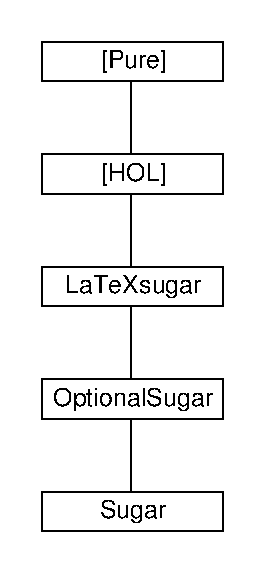
\includegraphics{session_graph}, in \texttt{document/root.tex} (omitting
the file-name extension enables {\LaTeX} to select to correct version, either
for the DVI or PDF output path).

\medskip The \texttt{-D} option causes the generated document sources to be
dumped at location \texttt{PATH}; this path is relative to the session's main
directory.  If the \texttt{-C} option is true, this will include a copy of an
existing \texttt{document} directory as provided by the user.  For example,
\texttt{isatool usedir -D generated HOL Foo} produces a complete set of
document sources at \texttt{Foo/generated}.  Subsequent invocation of
\texttt{isatool document Foo/generated} (see also \S\ref{sec:tool-document})
will process the final result independently of an Isabelle job.  This
decoupled mode of operation facilitates debugging of serious {\LaTeX} errors,
for example.

\medskip The \texttt{-p} option determines the level of detail for internal
proof objects, see also the \emph{Isabelle Reference
  Manual}~\cite{isabelle-ref}.

\medskip The \texttt{-v} option causes additional information to be printed
while running the session, notably the location of prepared documents.

\medskip The \texttt{-M} option specifies the maximum number of
parallel threads used for processing independent theory files
(multithreading only works on suitable ML platforms).  When tuning the
performance of large Isabelle sessions, the number of actual CPU cores
of the underlying hardware is a good starting point for option
\texttt{-M}.  The \texttt{-T} option determines the level of detail in
tracing output concerning the internal locking and scheduling in
multithreaded operation.  This may be helpful in isolating performance
bottle-necks, e.g.\ due to excessive wait states when locking critical
code sections.

\medskip Any \texttt{usedir} session is named by some \emph{session
  identifier}. These accumulate, documenting the way sessions depend on
others. For example, consider \texttt{Pure/FOL/ex}, which refers to the
examples of FOL, which in turn is built upon Pure.

The current session's identifier is by default just the base name of the
\texttt{LOGIC} argument (in build mode), or of the \texttt{NAME} argument (in
example mode). This may be overridden explicitly via the \texttt{-s} option.


\subsection*{Examples}

Refer to the \texttt{IsaMakefile}s of the Isabelle distribution's
object-logics as a model for your own developments.  For example, see
\texttt{src/FOL/IsaMakefile}.  The Isabelle \texttt{mkdir} tool (see
\S\ref{sec:tool-mkdir}) creates \texttt{IsaMakefile}s with proper invocation
of \texttt{usedir} as well.


\section{Preparing Isabelle session documents --- \texttt{isatool document}}
\label{sec:tool-document}

The \tooldx{document} utility prepares logic session documents, processing the
sources both as provided by the user and generated by Isabelle.  Its usage is:
\begin{ttbox}
Usage: document [OPTIONS] [DIR]

  Options are:
    -c           cleanup -- be aggressive in removing old stuff
    -n NAME      specify document name (default 'document')
    -o FORMAT    specify output format: dvi (default), dvi.gz, ps,
                 ps.gz, pdf
    -t TAGS      specify tagged region markup

  Prepare the theory session document in DIR (default 'document')
  producing the specified output format.
\end{ttbox}
This tool is usually run automatically as part of the corresponding Isabelle
batch process, provided document preparation has been enabled (cf.\ the
\texttt{-d} option of the \texttt{usedir} utility, \S\ref{sec:tool-usedir}).
It may be manually invoked on the generated browser information document
output as well, e.g.\ in case of errors encountered in the batch run.

\medskip The \texttt{-c} option tells the \texttt{document} tool to dispose
the document sources after successful operation.  This is the right thing to
do for sources generated by an Isabelle process, but take care of your files
in manual document preparation!

\medskip The \texttt{-n} and \texttt{-o} option specify the final output file
name and format, the default is ``\texttt{document.dvi}''.  Note that the
result will appear in the parent of the target \texttt{DIR}.

\medskip The \texttt{-t} option tells {\LaTeX} how to interpret tagged
Isabelle command regions.  Tags are specified as a comma separated list of
modifier/name pairs: ``\verb,+,$foo$'' (or just ``$foo$'') means to keep,
``\verb,-,$foo$'' to drop, and ``\verb,/,$foo$'' to fold text tagged as $foo$.
The builtin default is equivalent to the tag specification
``\texttt{/theory,/proof,/ML,+visible,-invisible}''; see also the {\LaTeX}
macros \verb,\isakeeptag,, \verb,\isadroptag,, and \verb,\isafoldtag, in
\texttt{isabelle.sty}.

\medskip Document preparation requires a properly setup ``\texttt{document}''
directory within the logic session sources.  This directory is supposed to
contain all the files needed to produce the final document --- apart from the
actual theories which are generated by Isabelle.

\medskip For most practical purposes, the \texttt{document} tool is smart
enough to create any of the specified output formats, taking \texttt{root.tex}
supplied by the user as a starting point.  This even includes multiple runs of
{\LaTeX} to accommodate references and bibliographies (the latter assumes
\texttt{root.bib} within the same directory).

In more complex situations, a separate \texttt{IsaMakefile} for the document
sources may be given instead.  This should provide targets for any admissible
document format; these have to produce corresponding output files named after
\texttt{root} as well, e.g.\ \texttt{root.dvi} for target format \texttt{dvi}.

\medskip When running the session, Isabelle copies the original
\texttt{document} directory into its proper place within
\texttt{ISABELLE_BROWSER_INFO} according to the session path.  Then, for any
processed theory $A$ some {\LaTeX} source is generated and put there as
$A$\texttt{.tex}.  Furthermore, a list of all generated theory files is put
into \texttt{session.tex}.  Typically, the root {\LaTeX} file provided by the
user would include \texttt{session.tex} to get a document containing all the
theories.

The {\LaTeX} versions of the theories require some macros defined in
\texttt{isabelle.sty} as distributed with Isabelle.  Doing
\verb,\usepackage{isabelle}, in \texttt{root.tex} should be fine; the
underlying Isabelle \texttt{latex} utility already includes an appropriate
{\TeX} inputs path.

If the text contains any references to Isabelle symbols (such as
\verb,\<forall>,) then \texttt{isabellesym.sty} should be included as well.
This package contains a standard set of {\LaTeX} macro definitions
\verb,\isasym,$foo$ corresponding to \verb,\<,$foo$\verb,>, (see
Appendix~\ref{app:symbols} for a complete list of predefined Isabelle
symbols).  Users may invent further symbols as well, just by providing
{\LaTeX} macros in a similar fashion as in \texttt{isabellesym.sty} of the
distribution.

For proper setup of PDF documents (with hyperlinks, bookmarks, and thumbnail
images), we recommend to include \verb,pdfsetup.sty, as well.  It is safe to
do so even without using PDF~\LaTeX.

\medskip As a final step of document preparation within Isabelle,
\texttt{isatool document -c} is run on the resulting \texttt{document}
directory.  Thus the actual output document is built and installed in its
proper place (as linked by the session's \texttt{index.html} if option
\texttt{-i} of \texttt{usedir} has been enabled, cf.\ \S\ref{sec:info}).  The
generated sources are deleted after successful run of {\LaTeX} and friends.
Note that a separate copy of the sources may be retained by passing an option
\texttt{-D} to the \texttt{usedir} utility when running the session (see also
\S\ref{sec:tool-usedir}).


\section{Running {\LaTeX} within the Isabelle environment --- \texttt{isatool latex}}
\label{sec:tool-latex}

The \tooldx{latex} utility provides the basic interface for Isabelle document
preparation.  Its usage is:
\begin{ttbox}
Usage: latex [OPTIONS] [FILE]

  Options are:
    -o FORMAT    specify output format: dvi (default), dvi.gz, ps,
                 ps.gz, pdf, bbl, png, sty, syms

  Run LaTeX (and related tools) on FILE (default root.tex),
  producing the specified output format.
\end{ttbox}
Appropriate {\LaTeX}-related programs are run on the input file, according to
the given output format: \texttt{latex}, \texttt{pdflatex}, \texttt{dvips},
\texttt{bibtex} (for \texttt{bbl}), and \texttt{thumbpdf} (for \texttt{png}).
The actual commands are determined from the settings environment
(\texttt{ISABELLE_LATEX} etc., see \S\ref{sec:settings}).

The \texttt{sty} output format causes the Isabelle style files to be updated
from the distribution.  This is useful in special situations where the
document sources are to be processed another time by separate tools (cf.\ 
option \texttt{-D} of the \texttt{usedir} utility, see
\S\ref{sec:tool-usedir}).

The \texttt{syms} output is for internal use; it generates lists of symbols
that are available without loading additional {\LaTeX} packages.


\subsubsection*{Examples}

Invoking \texttt{isatool latex} by hand may be occasionally useful when
debugging failed attempts of the automatic document preparation stage of
batch-mode Isabelle.  The abortive process leaves the sources at a certain
place within \texttt{ISABELLE_BROWSER_INFO}, see the runtime error message for
details.  This enables users to inspect {\LaTeX} runs in further detail, e.g.\ 
like this:

\begin{ttbox}
  cd ~/isabelle/browser_info/HOL/Test/document
  isatool latex -o pdf
\end{ttbox}


%%% Local Variables: 
%%% mode: latex
%%% TeX-master: "system"
%%% End: 


% $Id$

\chapter{Miscellaneous tools}

Subsequently we describe various Isabelle related utilities --- in
alphabetical order.


\section{Viewing documentation --- \texttt{isatool doc}} \label{sec:tool-doc}

The \tooldx{doc} utility displays online documentation:
\begin{ttbox}
Usage: isatool doc [DOC]

  View Isabelle documentation DOC, or show list of available documents.
\end{ttbox}
If called without arguments, it lists all available documents. Each
line starts with an identifier, followed by some comment. Any of these
identifiers may be specified as the first argument in order to have
the corresponding document displayed.

\medskip The \texttt{ISABELLE_DOCS} setting specifies the list of
directories (separated by colons) to be scanned for documentations.
The program for viewing \texttt{dvi} files is set in
\texttt{DVI_VIEWER}.


\section{Tuning proof scripts --- \texttt{isatool expandshort}}

The \tooldx{expandshort} utility tunes {\ML} proof scripts to enhance
readability a bit:
\begin{ttbox}
Usage: expandshort [FILES ...]

  Expand shorthand goal commands in FILES.  Also contracts uses of
  resolve_tac, dresolve_tac, eresolve_tac, rewrite_goals_tac on
  1-element lists; furthermore expands tabs, since they are now
  forbidden in ML string constants.

  Renames old versions of FILES by appending "~~".
\end{ttbox}
In the files supplied as arguments, all occurrences of the shorthand
commands \texttt{br}, \texttt{be} etc.\ are replaced with the
corresponding full commands.  Shorthand commands should appear one per
line.  The old versions of the files are renamed to have the
suffix~\verb'~~'.

\section{Get logic images --- \texttt{isatool findlogics}}

The \tooldx{findlogics} utility traverses all directories specified in
\texttt{ISABELLE_PATH}, looking for Isabelle logic images. Its usage
is:
\begin{ttbox}
Usage: isatool findlogics

  Collect heap file names from ISABELLE_PATH.
\end{ttbox}
The base names of all files found on the path are printed --- sorted
and with duplicates removed. Also note that \texttt{ISABELLE_PATH}
implicitely depends upon \texttt{ML_SYSTEM}. Thus switching to another
{\ML} compiler may change the set of logic images available.


\section{Inspecting the settings environment -- \texttt{isatool getenv}}
\label{sec:tool-getenv}

The Isabelle settings environment --- as provided by the site-default
and user-specific settings files --- can be inspected with the
\tooldx{getenv} utility:
\begin{ttbox}
Usage: isatool getenv [OPTIONS] [VARNAMES ...]

  Options are:
    -a           display complete environment
    -b           print values only (doesn't work for -a)

  Get value of VARNAMES from the Isabelle settings.
\end{ttbox}

With the \texttt{-a} option, one may inspect the full process
environment that Isabelle related programs are run in. This usually
contains much more variables than are actually Isabelle settings.
Normally output is a list of lines of the form
\mbox{$varname$\texttt{=}$value$}. The \texttt{-b} option causes only
the values to be printed.


\subsection*{Examples}

Get the {\ML} system identifier and the location where the compiler
binaries are supposed to reside as follows:
\begin{ttbox}
isatool getenv ML_SYSTEM ML_HOME
{\out ML_SYSTEM=smlnj-1.09}
{\out ML_HOME=/usr/local/sml109.27/bin}
\end{ttbox}

The next one peeks at the search path that \texttt{isabelle} uses to
locate logic images:
\begin{ttbox}
isatool getenv -b ISABELLE_PATH
{\out /home/me/isabelle/heaps/smlnj-1.09:/proj/isabelle/heaps/smlnj-1.09}
\end{ttbox}
We used the \texttt{-b} option to suppress the \texttt{ISABELLE_PATH=}
prefix.  The value above is what became of the following assignment in
the default settings file:
\begin{ttbox}
ISABELLE_PATH=\$ISABELLE_HOME_USER/heaps:\$ISABELLE_HOME/heaps
\end{ttbox}
Note how the \texttt{ML_SYSTEM} value got appended automatically to
each path component. This is a special feature of
\texttt{ISABELLE_PATH} (and also of \texttt{ISABELLE_OUTPUT}).


\section{Isabelle's version of make --- \texttt{isatool make}}

The Isabelle \tooldx{make} utility is a very simple wrapper for
ordinary Unix \texttt{make}:
\begin{ttbox}
Usage: isatool make [ARGS ...]

  Compiles logic in current directory using IsaMakefile.
  ARGS are directly passed to the system make program.
\end{ttbox}
Note that the Isabelle settings environment is also active. Thus one
may refer to its values within the \texttt{IsaMakefile}, e.g.\ 
\texttt{\$(ISABELLE_OUTPUT)}. Furthermore, programs started from the
make file also inherit this environment.

\medskip You may want to have a look at the \texttt{IsaMakefile}s of
the distributed object-logics as examples for your own developements.


\section{Running complete logics --- \texttt{isatool usedir}} \label{sec:tool-usedir}

FIXME

%FIXME
%    -g BOOL      generate theory graph data (default false)
\begin{ttbox}
Usage: isatool usedir LOGIC NAME

  Options are:
    -b           build mode (output heap image, use dir ".")
    -h BOOL      generate theory HTML data (default false)
    -s NAME      override session NAME

  Build object-logic or run examples. Also creates browsing
  information (HTML etc.) according to settings.
\end{ttbox}

FIXME


\appendix
\let\int\intorig

% $Id$

\chapter{Standard Isabelle symbols}\label{app:symbols}

Isabelle supports an infinite number of non-ASCII symbols, which are
represented in source text as \verb,\<,$name$\verb,>, (where $name$ may be any
identifier).  It is left to front-end tools how these symbols are presented to
the user.  The following predefined standard symbols are available by default
for Isabelle document output; most of these are also supported by
Proof~General when used together with the X-Symbol package.

Any symbol (or plain ASCII character) may be prefixed by \verb,\<^sup>, for
superscript and \verb,\<^sub>, for subscript; e.g.\ \verb,A\<^sup>\<star>, is
presented in {\LaTeX} as \isa{A\isactrlsup{\isasymstar}}.  Most symbols (and
all ASCII characters) may be printed in bold by prefixing \verb,\<^bold>,, as
in \verb,\<^bold>\<alpha>, which is printed as
\isa{\isactrlbold{\isasymalpha}}.  Note that super- and subscripts may
\emph{not} be combined with bold style.

See also Chapter~\ref{ch:present} for more details on Isabelle document
preparation.

\begin{center}
  \input{syms}  
\end{center}

%%% Local Variables: 
%%% mode: latex
%%% TeX-master: "system"
%%% End: 


\begingroup
  \bibliographystyle{plain} \small\raggedright\frenchspacing
  \bibliography{../manual}
\endgroup

\printindex

\end{document}
